

\section{Introduction}

The purpose of stance detection is to automatically find a relation type between specified sentences against a given text. So it is possible to evaluate what a news source is saying about a particular issue \cite{UCLMR}. The selected sentence could be a claim, a news item, an idea, a social network post, or any other source. Also, the text could retrieve from news agencies, weblogs, posts that are shared on social media, and any other available text. Choosing the source and context of sentences and texts depends on the goal of the defined task. Four considered labels are agreed, disagreed, discussed, and not enough information. 
\newline

Gathering a sufficient amount of data is a vital step to achieve reliable output. Both number of records in the data set and the quality of each sample have a significant effect on output accuracy. \cite{takestancefake}) gathered fifty thousand articles-headline pairs for their data set. (\cite{takestancefake}) achieved a respectable ninety percent accuracy, which was considerably higher than previous attempts by other researchers (\cite{book_fake}). In some contexts, there isn't enough available data. Here is where transfer learning methods play a vital role and compensate lack of data. We pre-trained a model on a large text corpus in a general context and then fine-tune the model on task-specified data. \cite{takestancefake} used RoBERTa model which is pre-trained on Facebook data. Then fine-tune it on the specific task at hand.
Also, \cite{stance_robust} improved its accuracy by fine-tuning BERT model.
\newline

Researchers have suggested various methods for stance classification. One cluster of methods mainly focuses on deep learning approaches. The precision of models is improved by using word embeddings such as BERT, using recurrent neural networks such as LSTM, BiLSTM (\cite{stanceCI}), attention-based network (\cite{stanceCI}). Some novel model architectures are currently proposed, such as Memory Network (\cite{memory_network}).
\newline

One possible way of evaluating the accuracy of a given claim is detecting the stance of that claim against available trusted sources. Stance detection task traditionally were used in political and ideological debates fields \citep{stance_robust}.The idea of using Stance Detection techniques to analyze news items' correctness has become caught researcher's attention since 2016. Consistency of a sentence through sources can be retrieved by stance detection methods. Stance detection can be considered as a subtask of fake news detection (\cite{book_datafake}). It is easier to judge a claim by its stance against other sources. So estimating the stance of a particular claim against available documents can be the first step into detecting fake news. 

\section{Literature Review}
\label{literature}
	Many researches have done to improve stance detection accuracy. Different ideas and architectures has applied. In the following part, previous research and papers has been over viewed. 
	\newline 
	
	On 2016 \cite{Augenstein2016StanceDW} started working on the challenging task without assuming neither target is clearly mentioned in the text nor training date is given for every target. Their dataset construct of tweets, mostly contains politicians and popular issues. \cite{Augenstein2016StanceDW} used conditional LSTM encoding on Tweeter data, And results are even improved by using bidirectional encoding. Using LSTM-based models lead to better result rather than Majority class, SVM and BoWV baseline in this experiment. This paper mainly focus on detect stance with respect to unseen targets. This paper included that using unconditional LSTM work best for unseen targets.
	
	 \cite{UCLMR} has developed an stance detection end-to-end system including lexical and similarity-based featured which is passed through a multi-layer perception model. UCLMR's\footnote{UCL Machine Reading} model claimed third place in FNC-1\footnote{First stage of a competition Fake News Challenge(FNC-1) is exploring how artificial intelligence technologies could be leveraged to combat fake news\footnote{fakenewschallenge.org}. Numerous researchers has interest in this field and many papers has published besides this challenge.}. UCLMR's model architecture is illustrated on Figure \ref{fig:UCLMR-system}. Headline and body texts are tokenised by sikit-learn\footnote{\cite{sikit-learn}}. Furthermore, \cite{UCLMR} used both term frequency (TF) vector of headline and claim and cosine similarity between head and body $l$2-normalised TF-IDF vectors. Besides, stop words are excluded. \cite{UCLMR} achieved FNC-1 score of 75.20\% on the test data set.
	\begin{figure}
		\centering
		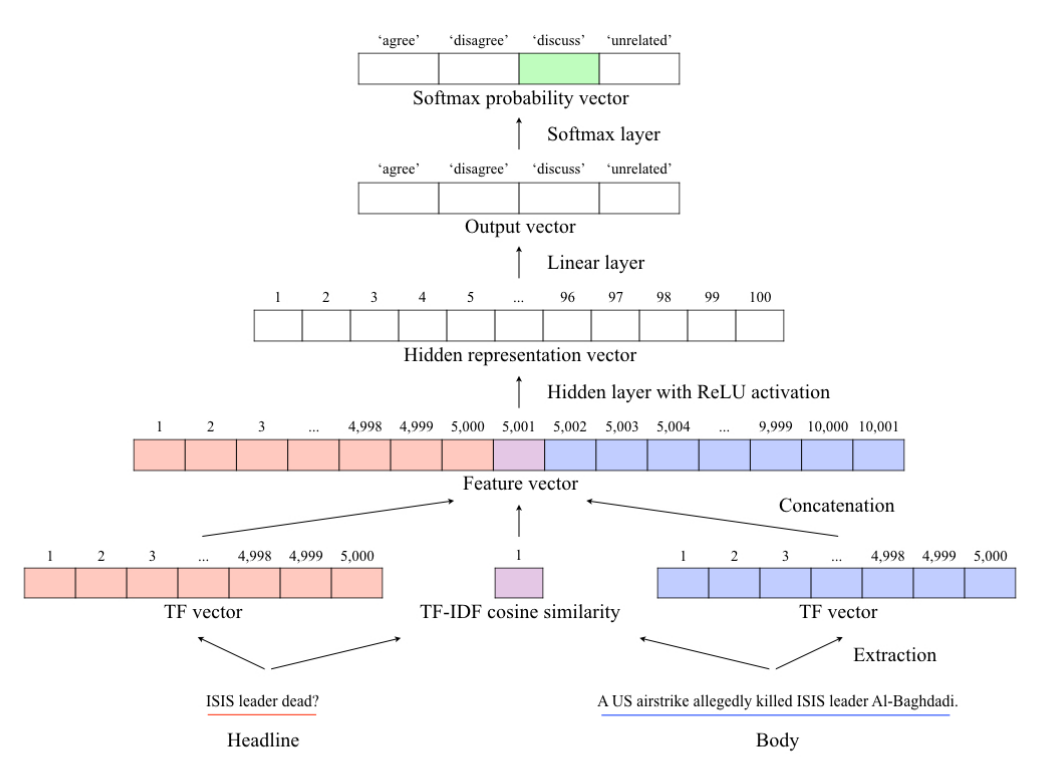
\includegraphics[scale=0.4]{statistics/stance/simple-baseline-FNC.png}
		\caption{Schematic diagram of UCLMR’s system.}
		\label{fig:UCLMR-system}
	\end{figure}


	\cite{Hierarchical-Attention-Network} has mainly focused on linguistic information such as polarity and argument of the document to represent a document. As it is shown in \ref{fig:hierarchical_att} document, sentiment, dependency, and argument representations are used in model architecture. \cite{Hierarchical-Attention-Network} concluded that every linguistic information with attention mechanism improves stance detection, And using linguistics features all together outperform using them individually. More explanation is available in the following lines. 
	
	\begin{itemize}
		\item \textbf{Document Representation}: Use LSTM model to represent each document.
		\item \textbf{Sentiment Representation}: As sentiment representation LSTM model is used to learn the the representation of sentiment information.The sentimental word sequence of each document is extracted from sentiment lexicon. 
		\item \textbf{Dependency Representation}: This feature is used to capture inter-word relationships. Extract relation from dependency parser. Finally learn representation of dependency sequence, using a LSTM layer.
		\item \textbf{Argument Representation}: Argument is considered as author's stance. \cite{Hierarchical-Attention-Network} used a binary classification to detect the document's argument sentence, then learn the sequence representation of word sequence in argument sentences utilizing LSTM layer.
	\end{itemize}
	
	In addition, it utilized a hierarchical attention network in order to weigh the importance of linguistic information, and learn the mutual attention between the document and linguistic information. \cite{Hierarchical-Attention-Network} mentioned that Hyper Attention layer in Figure \ref{fig:hierarchical_att}, had a considerable influence on model performance. 
	
	\begin{figure}
		\centering
		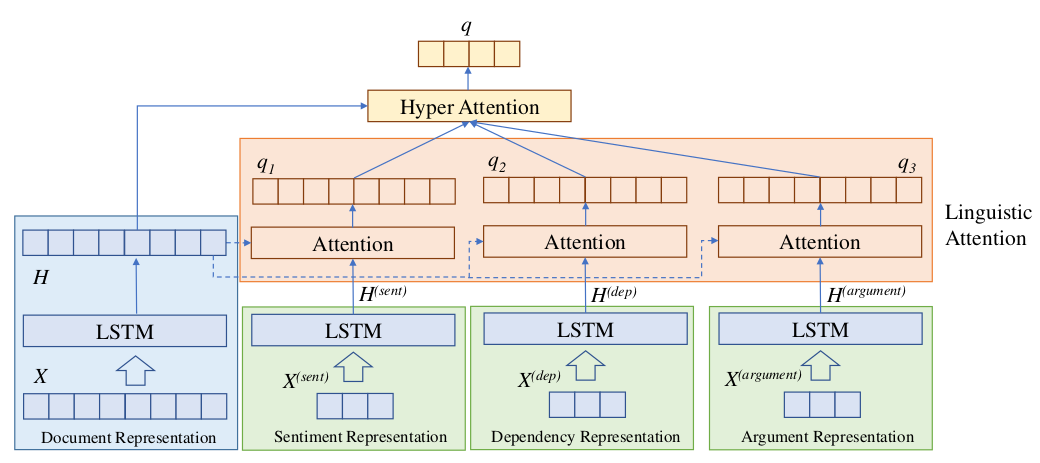
\includegraphics[scale=0.4]{statistics/stance/hierarchial-attention-network.png}
		\caption{Overview of \cite{Hierarchical-Attention-Network} model.}
		\label{fig:hierarchical_att}
	\end{figure}
	
	\cite{memory_network} present a novel end-to-end memory network on 2018 to predict stance and extract snippet of the prediction. Model mainly focus on relevant paragraphs. It compute . This model incorporate recurrent and convolutional neural networks and similarity matrix. \cite{memory_network} mentioned that detecting \emph{disagree} is the hardest label to predict. To overcome unbalancing issue, \cite{memory_network} select the same number from each class in each iteration. 
	\begin{figure}
		\centering
		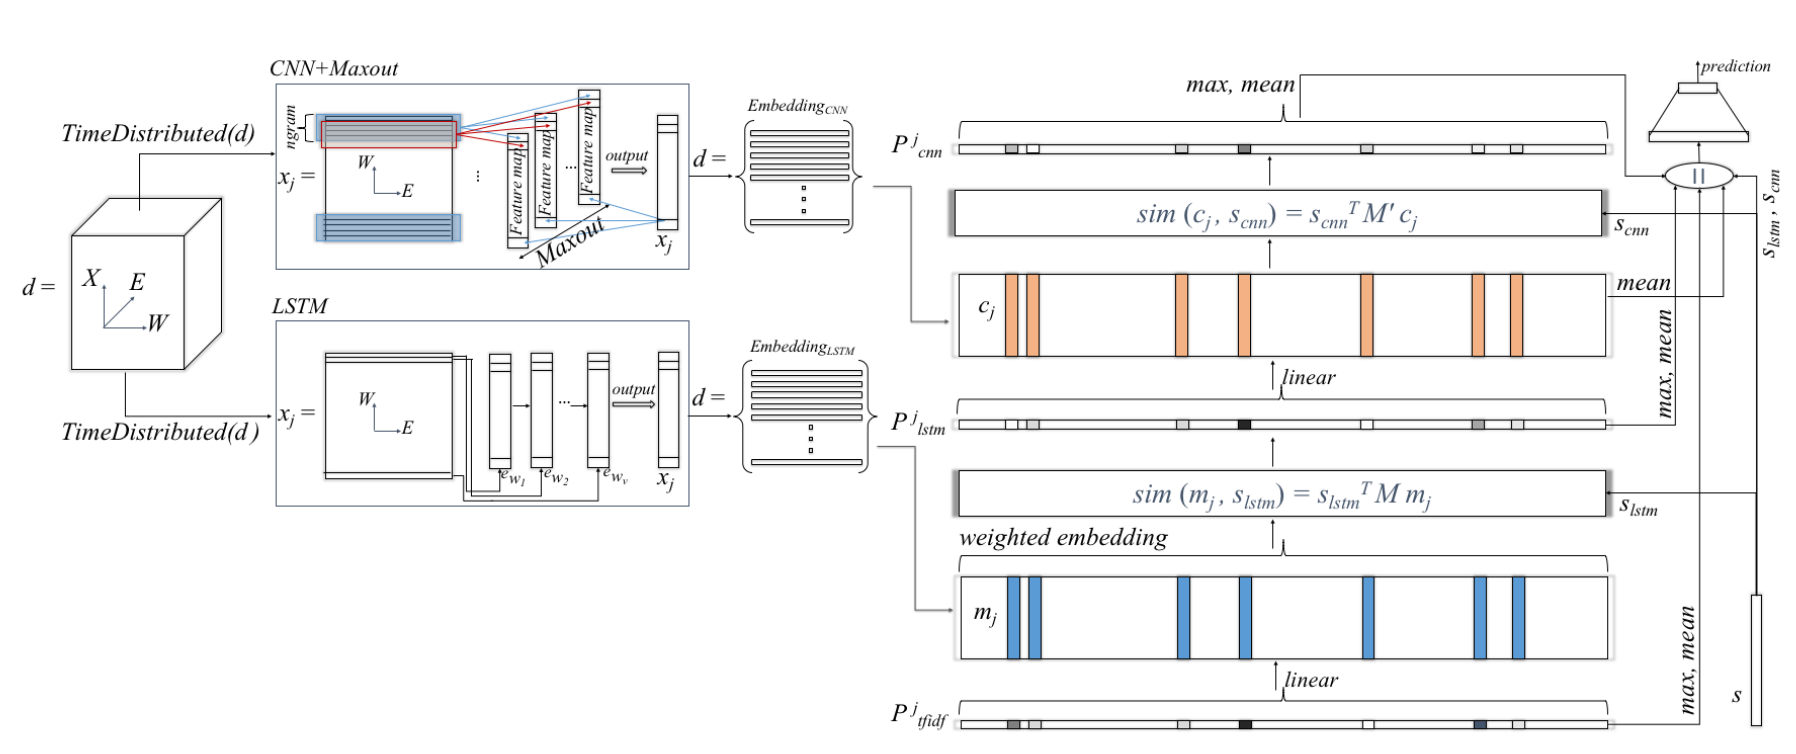
\includegraphics[scale=0.25]{statistics/stance/memoty_network.png}
		\caption{Architecture of Memory Network for stance detection.}
		\label{fig:mem_network}
	\end{figure}

	\cite{stance_robust} mainly focused on robustness of a stance detection classifier. Models trained on a single data set in a special domain, won't robust enough on other domains. So they suggested using multi-domain dataset or use mutli-dataset learning methods to improve model generalization. Model architecture is construct of fine-tuned BERT\cite{bert} and single dense classifier at the top. \cite{stance_robust} used 5 fixed seed value during training nd reported averaged results. \cite{stance_robust} concluded that MDL(multi-dataset learning) has significant impact on increasing model robustness.
	
\section{Dataset}
\label{sec:dataset}
First Persian stance detection dataset (\cite{stance_persian})  is used in this project. \cite{stance_persian} dataset can be used in stance detection, summarization and fake news detection tasks. This dataset contains 2124 news article, covering information about 534 claim. Number of each sample is specified in table \ref{tbl:sdatapie}. Claims are retrieved from Shayeaat \footnote{shayeaat.ir} and Fakenews\footnote{fakenews.ir} websites. Each samples contains 3 different labels for stance detection task, containing article's headline toward the claim, article's body toward the claim and article's headline toward it's body. Samples are tagged manually. Four following classes is considered for stance classifying:
\begin{itemize}
	\item {\color{green!70!black}\textbf{Agree:}} The article clearly states that claim is True without any ambiguity or amphibology. 
	\item {\color{red!70!black}\textbf{Disagree:}} The article clearly refutes the claim without any ambiguity or amphibology. 
	\item {\color{yellow!70!black}\textbf{Discuss:}} The article contains information about the claim but don't have any evaluation on it's truth. 
	\item {\color{gray!}\textbf{Unrelated:}} There isn't any information about the claim in the article.
\end{itemize}
Dataset samples distribution in each classes is illustrated in Figure \ref{fig:datacom}. According to Figure \ref{fig:datacom}, ration of \textit{Agree} and \textit{Disagree} labels are much lower than the others and there is potential risk for models to be bias on \textit{Unrelated} and \textit{Discuss}. Also, percentage of \textit{Unrelated} label is higher in headline to claim than article to claim. Headline can be considered as a summary of news body so unlike news text, news headline may not have enough information to evaluate a claim.  Besides ratio of \textit{Discuss} to \textit{Agree} and \textit{Disagree} is higher in Article to claim than headline to claim. It seem that news agencies choose more controversial headlines to appeal reader's attention.

Furthermore this dataset covers each claim veracity according to related news articles. In this dataset, main focus has been on fake news, This can be inferred from figure \ref{fig:fake}. Three following labels are considered for classifying news veracity:


\begin{itemize} 
	\item {\color{green!70!black}\textbf{True16:}} Reliable news agencies have asserted that this claim is a fact.
	\item {\color{red!70!black}\textbf{False120:}} Unreliable news agencies have spread data about this claim and reliable news agencies have considered this claim as a hearsay.
\item {\color{gray}\textbf{Unknown5:}} There isn't enough integrity between reliable news agencies sources.
\end{itemize}




\begin{table}
	\centering
	\caption{Class distribution}
	\begin{tabularx}{0.8\textwidth} { 
			| >{\centering\arraybackslash}X 
			| >{\centering\arraybackslash}X 
			| >{\centering\arraybackslash}X 
			| >{\centering\arraybackslash}X 
			| >{\centering\arraybackslash}X | }
		\hline
		Label & Agree & Disagree & Unrelated & Discuss \\
		\hline
		Headline to claim & 628  & 210  & 932 & 824  \\
		\hline
		Article to claim & 189  & 374  & 797 & 1196  \\
		\hline
		
	\end{tabularx} 
	\label{tbl:sdatapie}
\end{table}

\begin{figure}%
	\centering
	\subfloat[\centering Artcile to Claim]{{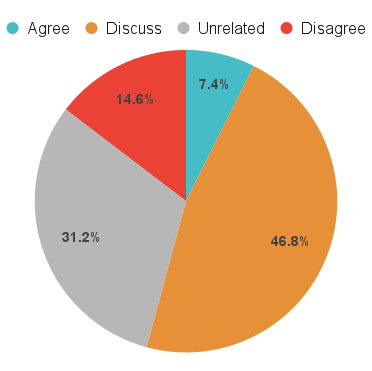
\includegraphics[width=6cm]{statistics/stance/a2c.png} }}%
	\qquad
	\subfloat[\centering Headline to claim ]{{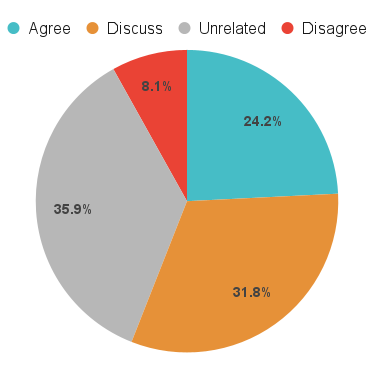
\includegraphics[width=6cm]{statistics/stance/h2c.png} }}%
	\caption{Comparison between Article to claim and Headline to claim labels, samples distribution in \cite{stance_persian} dataset.}%
	\label{fig:datacom}%
\end{figure}
\begin{figure}%
	\centering
	{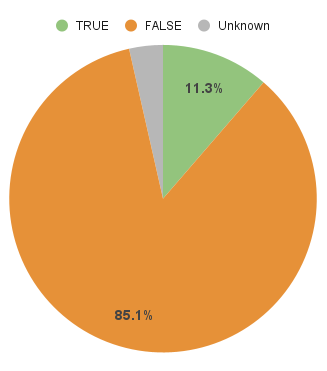
\includegraphics[width=5.5cm]{statistics/stance/fake.png} }
	\caption{Claim veracity label's distribution in \cite{stance_persian} dataset.}%
	\label{fig:fake}%
\end{figure}
  
\section{Experiments}
The headline of news is a summary of its body content and most of the time, it carries valuable data. So, we focused on detecting the news headlines stance towards claim(H2C), as well as the news articles stance towards a claim(B2C). According to the lower amount of text in the news headline, most of the experiments are firstly applied on H2C then, better approaches are applied on A2C.  
\subsection{Preprocessing}
First and mandatory preprocessing step, is to tokenize words in corpus in order to remove and detect special words. Four different following tokenizer performance on Persian language has evaluated. 
\begin{itemize}
	\item \textbf{Hazm\footnote{sobhe.ir}:}
	Hazm is a python library Persian language processing tool kit. It has variety of function such as word and sentence tokenizer, word lemmatizer, POS tagger, Shallow and Dependency parser.
	
	\item \textbf{NLTK\footnote{nltk.org}:}
	NLTK (Natural Language ToolKit) is a python platform to work easier with human language data. This tool kit supports more than 50 corpus and supports numerous languages including Persian. 
	
	\item \textbf{Stanford\footnote{stanfordnlp.github.io/stanza}:}
	Stanford NLP tools is also another useful NLP tools package which currently switched to \textit{Stanza}. It is efficient for linguistic analysis and supports more than 70 human languages and releases new versions constantly.
	
	\item \textbf{BERT\footnote{huggingface.co/transformers/main\_classes/tokenizer.html}:}
	BERT (\cite{bert}) is a transformer based machine-learning model which is currently used in various natural language processing tasks. Persian pre-trained BERT model\footnote{huggingface.co/HooshvareLab/bert-base-parsbert-uncased} can be used for tokenizing corpus too. 
\end{itemize}

It is vital in tokenizing step to break corpus in to correct words. It may happens that tokenizers generate meaningless words, this is why tokenizers limit number of accepted words. Also, sometime tokenizers haven't seen words before, and omit them while tokenizing a corpus. According previous reasons it is important too choose tokenizer carefully.


After tokenization, list of punctuation and Persian stop-words are considered as \textit{denied} and will remove from corpus in this step. Firstly, same stop-words was used which have been used by \cite{stance_persian}, After reviewing preprocessed corpus, it was hard to infer from text pieces, So we chose stop-words carefully in a way not to loose refuting or supporting expressions. Kharazi\footnote{\label{fn:kharazi}github.com/kharazi/persian-stopwords} has classified stop-words into verbal, nonverbal and short. Verbs carries valuable information in news. Nonverbal stop-word class is a better choice to remove low value words in this task. Besides some keywords in news fields are removed from Kharazi's\footref{fn:kharazi} gathered stop-words. 

Also English number characters will remove from corpus before tokenizing. After preprocessing tokens, all tokens will be concatenated with space character and considered as prepossessed and clean corpus.


\subsection{Word Representation}
To represent a corpus, tokens should be converts to vector. Good vectors have to carry semantic word or n-grams, sequential words contents, and be as brief as possible. As a baseline three different Bag-of-word (\cite{bow}), TF-iDF (\cite{tfidf}), and Word-to-Vector (\cite{word2vec}) algorithms are evaluated. 

\subsubsection{BoW\protect\footnote{en.wikipedia.org/Bag-of-words\_model}}
Bag-of-Words (\cite{bow}) model, is a way to represent text. BoW keeps words frequency and
dismisses word's orders. Dimension of text representation is equal to number of specified words plus one for words that don't exist in specified words. Each cell in output text representation stands for a specific words and value of that cell is equal to number of repetition in that particular text. As an alternative, it is possible to choose n-gram instead of single word as BoW dictionary. This may improve BoW model in order to keep longer expression semantic but on the other hand dimension of representation exceed vastly. Disadvantages of this model are it doesn't specify any relation between words with similar semantic meaning. 

\subsubsection{TF-IDF}

Term Frequency–Inverse Document Frequency (\cite{tfidf}) is an algorithm to present importance of each word in a corpus in statistics way. According to repetition of a specific word in each document and ... a float number will be assign to each word in that corpus.  
\begin{itemize}
	\item \textbf{Trem frequency (TF):} This item represents how many times a words used in each documents. \textit{TF} should be calculate for each document separately. \textit{TF} term calculate from equation \ref(tf)
	\begin{equation}
	\label{tf}
		tf \left(t,D\right) = \frac{f_{t,d}}{\Sigma_{t^{`} \in d } f_{t^{`}, d}}
	\end{equation}
	
	\item \textbf{Inverse Document Frequency (iDF):} This term present how much information a word have. The less repetition of a word through documents, the more information it has. This term is calculated from equation \ref{idf}. 
	\begin{equation}
	\label{idf}
		idf \left( t,D\right) = \log \frac{N}{\left|\{d\in D, t \in d\}\right| }
	\end{equation}
\end{itemize}

\noindent
After calculating \textit{TF} and \textit{iDF}, TF-iDF value for each word calculate from equation \ref{tfidf}.
\begin{equation}
	\label{tfidf}
	tf-idf\left(t,d,D\right) =  tf \left( t,D\right) . idf \left( t,D\right)
\end{equation}


\subsubsection{W2V\protect\footnote{en.wikipedia.org/wiki/Word2vec}}
Word2vec (\cite{word2vec}) is a neural network based model which learns each word semantic and even it can recommend words with similar meaning to a specific word. Word2Vec represents each word with a vector instead of a number. After training phase, each word vector serve numbers that is generally similar to words with similar meaning and words with less similarity have lower vector similarities. This vector is called word-embedding. It is necessary to have large corpus in order to have a powerful model which can predict each word vector precisely. Multiple alternative algorithm for Word2Vec exist. In this project FastText\footnote{fasttext.cc} Word2Vec model is used with vector length equal to 300 which is trained on Persian Wikipedia website. Fasttext is an extension of Word2Vec model which treat each words as concatenated n-grams.  


\subsection{Features}
\label{sec:features}
\subsubsection{Similarity}
Similarity score is offered by \cite{stance_persian}. This feature calculates how much a claim is similar to a headline or a news article, depends on the task. Three following sequence matching score is considered for this feature by utlizing \textit{difflib}\footnote{docs.python.org/3/library/difflib.html} python library.

\begin{itemize}
	\item Ratio: Similarity score in float range 0,1. This paramets calcualtes from equation \ref{eq_ratio}
	\begin{equation}
		\label{eq_ratio}
		ratio = \frac{2.0 * M}{T}
	\end{equation}
	where:
	\begin{eqexpl}[25mm]
		\item{$T$}Number of elements in both sequences.
		\item{$M$}Number of matches.
	\end{eqexpl}
	\item Quick Ratio: This parameter estimate an upper bound on Ratio.
	\item Real Quick Ratio: This parameter estimate an upper bound on Ratio.
\end{itemize}
\subsubsection{Root Distance}
This feature is suggested by \cite{stance_persian}. Root Distance stands for distance between root of a headline and some collected hedge, refuting and reporting words. Firstly, set of words which considered as mentioned group are gathered and then for each word distance is calculated.
%\newline{\color{red}=================TODO========================}
\subsubsection{ImportantWords}
List of controversial and challenging word in news are gathered by \cite{stance_persian} and considered as \textit{important-words}. This feature is a zero based list with the length of important words, and each cell stands for one word in \textit{important-words}. List carries number of repetition of desire words in a specific news article.
\subsubsection{Is Question}
Is-Question identifies whether a claim or headline a news article ends with question marks or not. \cite{stance_persian} dataset contains a column dedicated to this feature.
\subsubsection{Has Two Parts}
Has-Two-Parts is if a claim is construct of two separately parts. \cite{stance_persian} dataset contains a column dedicated to this feature.
\subsubsection{Polarity}  
Polarity of a text can be utilized in variety of tasks. This feature presents how positive or negative a text is. Different algorithm are developed to predict polarity of a text. In this project \cite{persent} dataset is used to calculate each sample sentiment. \cite{persent} contains dictionary of words with their sentiment score between -1 and 1. The more negative meaning a word has, the less value it's polarity has. For each word presents in each sample at most first 30 nonzero polarity value saves in a zero initialed vector with 30 length. As \cite{persent} contains only 1500 word polarity values, it can't cover all words in corpus and it has far way to improve. 

In this project an idea is applies to extend PerSent (\cite{persent}) polarity dataset is to use a language model. It is possible to predict similar words with a particular word and estimate their similarity score with a language model. Firstly, similar words that don't polarity score in PerSent with their similarity scores extract from a pre-trained language model. Then search each word in PerSent dataset and apply equation \ref{eq_polar} average through all similar words polarity score, to estimate the desired word polarity score.

\begin{equation}
	\label{eq_polar}
	polarity\_score\left(w\right) = \frac{\Sigma_{w^{`} \in W} Similatiry\left(w^{`}, w\right) . Polarity\left(w^{`}\right)}{\Sigma_{w^{`} \in W} Similatiry\left(w^{`}, w\right)}
\end{equation}

where: 
\begin{eqexpl}[25mm]
	\item{$w$}Desire word $\notin$ PerSent datast.
	\item{$W$}Similar words, Predicted by the language model
	\item{$Similarity$}Similarity score for 2 words which is predicted by the language model.
	\item{$polarity$} Polaroty score which is estimated by \cite{persent} dataset.
\end{eqexpl}

\bigbreak
One alternative is to use deep neural networks model to predict polarity whether word-level or sentence-level. But due to lack of Persian dataset in this context it is not possible. Available datasets for sentiment analysis are mainly gathered from costumer comments on special businesses. For instance \cite{polar_hotel} used 2 different dataset, first it translated English sentiment analysis corpus and second used comments on hotel. \cite{polar_servic} used dataset from SnappFood\footnote{snappfood.ir}, DigiKala\footnote{digikala.ir} comments. One main problem with these datasets are difference use of language between users comments and news. Users mostly use everyday language on the other hand news agencies use formal language.
\subsection{Machine Learning}
Machine learning algorithms aim to learn patterns on a corpus of data while training procedure, then predict class of new test data by those patterns (\cite{book_fake}). Machine learning algorithms have powerful performance even in complex problems. Machine learning algorithms in compare to deep learning models learn patterns according to its fed manually extracted predictors, and we don't have any other choice rather than relying on those number of extracted predictors (\cite{book_fake}). So extracting useful features  is a critical step in machine learning. The more meaningful and suitable predictors they see for a task, the better patterns they can find during training procedure. Performance of each predictor described in section \ref{sec:features}, is evaluated by following machine learning methods.   

\subsubsection{Gaussian Naive Bayes}
First machine learning algorithm used to classify stance is Gaussian Naive Bayes Classifier (\cite{GNbayes}). It is an alternative to machine learning Naive Bayes classifier that inspires from Bayes Theorem\footnote{en.wikipedia.org/wiki/Naive\_Bayes\_classifier}:

\[ P\left(y | X\right) =   \frac{P(X|y).P(X)}{P(y)} \]
where:
\begin{eqexpl}[25mm]
	\item{$X$} List of predictors that are independent to each other.
	\item{$y$} Label of a class.
	\item{$P\left(X|y\right)$} Probability of class with label $y$ from given X predictors.
\end{eqexpl}
 Naive Bayes Classifier algorithm estimates probability of each class. Gaussian Naive Bayes means that predictors are continuous and follow Gaussian distribution:
 
 \[p\left(x=\upsilon | C_{k}\right) = \frac{1}{\sqrt{2\pi\sigma_{k}^{2}}}e^{-\frac{\left(\epsilon-\mu_{k}\right)^{2}}{2\mu^{2}_{k}}}\]
\begin{eqexpl}[25mm]
	\item{$C_{k}$} Class k.
	\item{$\mu_{k}$} Mean of $x$ values associated with $C_{k}$
	\item{$\sigma^{2}_{k}$} Bessel corrected variance x values associated with $C_{k}$
\end{eqexpl}

\subsubsection{SVC\protect\footnote{wikipedia.org/Support-vector\_machine}}
\label{SVM}
SVC stands for SVM classifier. Support Vector Machines (\cite{svc})  are group of supervised machine learning models. One of their application is classification. SVM algorithms map each sample to a space that each class samples be as far as possible from other class samples. In the other word SVM id looking for a n-dimensional hyperplane which can separate classes as clearly as possible.

SVC model from \textit{scikit-learn}\footnote{scikit-learn.org/stable/modules/generated/sklearn.svm.SVC.html} python library is used in this project. Regularization parameter ($ c $) which is stands for strength of regularization is set to 10. As a kernel three different \textit{rbf}, \textit{sigmoid}, and \textit{poly} hyperplane are evaluated. Kernel specifies the type of separator that SVM algorithm use to distinguish different classes. Furthermore, \textit{class\_weight} parameter set to \textit{balanced} which mean set different weight for each class during training to compensate imbalanced data. 


\subsubsection{LinearSVC}
LinearSVC is a ulternative algorithm for SVC in large datasets. LinearSVC linearly separates samples. Depends on dataset it may works better than nonlinear SVC. This model is same as SVC from previous part, only different is to set \textit{kernel} parameter equal to linear. 
 
\subsubsection{Random Forest}
Random Forest (\cite{randomforest}) is a machine learning algorithm to deal with complex classification problems. It construct of many decision trees. The point is that it is more robust than decision threes. Besides Random Forest classifier doesn't need parameter tuning. Each decision three has it's own prediction and final prediction of the model is calculated bt majority voting of each tree output. 

In this project, implemented Random Forest algorithm from \textit{scikit-learn}\footnote{scikit-learn.org/stable/modules/generated/sklearn.ensemble.RandomForestClassifier.html} python library is used. Two parameters of \textit{max\_depth} and \textit{min\_samples\_leaf} control size of each decision tree. They are respectively set to 10 and 1. \textit{min\_samples\_split} bounds least number of samples to apply on a tree, is set to 3. 

\subsubsection{Logistic Regression}
Logistic Regression is a machine learning classification algorithm. It's functionality is mainly for Binary Classification and In multi-class Logistic regression classifies, one class vs rest. This algorithm uses 'Sigmoid function' as it's cost function and its prediction is based on probabilities. 

Implemented Logistic Regression algorithm from \textit{sckiti-learn}\footnote{scikit-learn.org/stable/modules/generated/sklearn.linear\_model.LogisticRegression.html} python library is used. \textit{penalty} parameter could be choosed from \textit{l1}, \textit{l2}, and \textit{elasticnet} for penalization and regularization.
\begin{itemize}
	\item $l1$
		\[ min_{\omega,c} \; \frac{1}{2}\omega^{T}\omega + C \Sigma_{i=1}^{n} \log\left(\exp\left(-y_{i}\left(X^{T}_{i}\omega + c \right)\right) + 1 \right) \]
	\item $l2$
		\[ min_{\omega,c} \; \left|\left|\omega\right|\right|_{1} + C \Sigma_{i=1}^{n} \log\left(\exp\left(-y_{i}\left(X^{T}_{i}\omega + c \right)\right) + 1 \right) \]
	\item $elastic-net$
		\[ min_{\omega,c} \; \frac{1-\rho}{2}\omega^{T}\omega +\rho\left|\left|\omega\right|\right|_{1} + C \Sigma_{i=1}^{n} \log\left(\exp\left(-y_{i}\left(X^{T}_{i}\omega + c \right)\right) + 1 \right) \]
\end{itemize}
where:
\begin{eqexpl}[25mm]
	\item{$\rho$} Controls $\; l1 \;$ strength (\textit{l1\_ration} parameter).
	\item{$y_{i}$} Takes value between -1, 1.
\end{eqexpl}
\bigbreak
Elastic-Net Penalization is used with $\; \rho \;$ parameter equals to 0.5, means $\;l1\;$ and $\;l2\;$ have same powers and \textit{solver} parameter which stand for optimizer algorithm is set to \textit{sega} which is an alternative for Stochastic Average Gradient (sag) optimizer. 

Another configuration for Logistic Regression is also evaluated. In this setup, optimizer is set to \textit{lbfgs} which performs more robust in larger datasets. Although, \textit{lbfgs} optimizer is slower than \textit{saga}.  Also, penalization is set to $\; l2 \;$\footnote{scikit-learn.org/stable/modules/linear\_model.html\#logistic-regression}.

\subsection{Balancing}
As mentioned in section \nameref{sec:dataset}, Figure \ref{fig:datacom}, number of samples in dataset classes was imbalanced. As a result, models bias on majority class and there may not enough sample in minority class for model to learn that, this leads to having high accuracy score (Equation \ref{eq:acc}) while having low f1 score (Equation \ref{eq:f1}).  
\begin{equation}
\label{eq:acc}
F1 = \frac{TP + TN }{TP + FN + TN + FP}
\end{equation}
where:
\begin{eqexpl}[25mm]
	\item{$TP$} True Positive
	\item{$TN$} True Negative
	\item{$FP$} False Positive 
	\item{$FN$} False Negative
\end{eqexpl}

\begin{equation}
	\label{eq:f1}
	 F1 = \frac{2 \times precision \times recall }{precission + recall}
\end{equation}
where: 
\begin{eqexpl}[25mm]
	\item{$precission$} $\; precision = \frac{TP}{TP + FP} \;$
	\item{$recall$} $\; recall = \frac{TP}{TP + FN} \;$ 
\end{eqexpl}

\bigbreak
There are several algorithm to deal with imbalanced datasets. In \cite{stance_persian} minority class forms only 7.4\% of data (Figure \ref{fig:datacom}). So it's not practical to rely on only one method and except to perform in the best way. Consecuently, three different methods used in this project in order to dealing with this phenomenon. Methods of balancing dataset which are used in this project is described in following sections.  
	
\subsubsection{\textbf{Extending dataset:}}
The simplest method is to gather data for classes except majority class. But unfortunately it is not always practicable. Another way of extending dataset is to use another existing dataset which has similar gathering logics and it is possible to map these two dataset classes. 

ParsFEVER (\cite{parsfever}) is a persian dataset set based on FEVER (\cite{fever}) dataset is gathered for fact extraction and verification task. \cite{parsfever} claims are generated from Wikipedia\footnote{wikipedia.org} articles manually, then evidences for each claim are extracted from Wikipedia separately by distinct annotators. This dataset contains three \textit{Support}, \textit{Refute}, and \textit{Not Enough Info} classes. 
\begin{itemize}
	\item {\color{green!70!black}\textbf{Support:}} The article obviously proves the given claim. 
	\item {\color{red!60!black}\textbf{Refute:}} The article obviously disproves the given claim.
	\item {\color{gray}\textbf{Not Enough Info:}} There isn't enough information in the article about the claim. 
\end{itemize}                

According to Figure \ref{fig:datacom} two \textit{Agree} and \textit{Disagree} class in \cite{stance_persian} dataset suffers from lack of samples. In this project, \textit{Supports} and \textit{Refutes} samples from \cite{parsfever} dataset are mapped to \textit{Agree} and \textit{Disagree} class of \cite{stance_persian} dataset respectively. 
But it is not possible to extend \textit{Discuss} or \textit{Unrelated} class by ParsFEVER, because they are both merged in \textit{Not Enough Info} class. As a result, two \textit{Agree} and \textit{Disagree} extended as much as possible with random selected samples from ParsFEVER dataset. Sample distribution is illustrated in figure \ref{fig:datab1}. Dataset is still imbalanced in one class for both Article to Claim and Headline to Claim.

\begin{figure}%
	\centering
	\subfloat[\centering Artcile to Claim]{{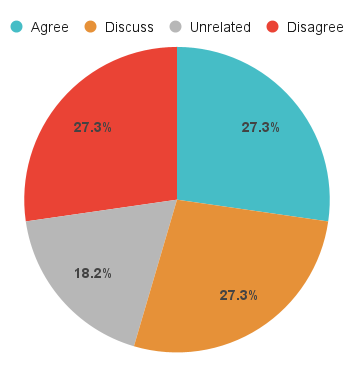
\includegraphics[width=6cm]{statistics/stance/a2c_b1.png} }}%
	\qquad
	\subfloat[\centering Headline to claim ]{{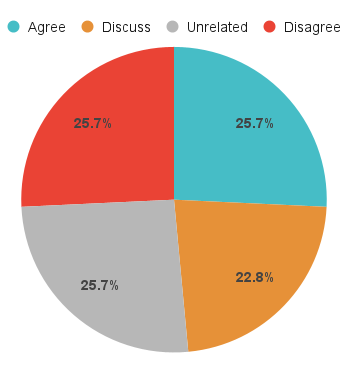
\includegraphics[width=6cm]{statistics/stance/h2c_b1.png} }}%
	\caption{Comparison between Article to claim and Headline to claim labels, samples distribution in \cite{stance_persian} dataset, after extending by \cite{parsfever} .}%
	\label{fig:datab1}%
\end{figure}

\subsubsection{\textbf{Oversampling and Undersampling:}}
 Another common way of dealing with imbalanced dataset is automatically augmenting samples to achieve balanced class distribution (Oversampling) or even reduce number of samples in majority class (Undersampling). Undersampling is applicable on large dataset. But in small dataset it's not wisely to ignore some samples. Oversampling methods suites for such datasets. According figure \ref{fig:datab1} Despite extending dataset with \cite{parsfever} dataset, balancing dataset is still needed. Though, oversamping shoud be performed on minority class only. It is important to split test and train sets before resampling, and oversampling should be only apply on train set. Resampling methods that evaluated are: 
\begin{itemize}
	\item \textbf{RandomOverSampler\footnote{imbalanced-learn.org/stable/references/generated/imblearn.over\_sampling.RandomOverSampler.html}:} This method randomly peak samples from classes and resample them. Random Over Sampler is the most naive algorithm and its performance is same as increasing minority class loss weight. Another variant of this method is smoothed bootstrap oversampling. It is generally similar to Random Oversampler, but new samples don't exactly overlap original samples. They are adjacent to source samples. This variant can be implement by \textit{shrinking} parameter in \textit{RandomOverSampler} from \textit{imblearn} python library. 
	
	\item \textbf{SMOTE:} 
	Synthetic Minority Over-sampling Technique (\cite{smothe}) is an oversampling method by generating new samples by interpolation. It's not important for smothe sampler that which point is choosed to be resampled. 
	
	\item \textbf{SVMSMOT\footnote{imbalanced-learn.org/stable/references/generated/imblearn.over\_sampling.SVMSMOTE.html}:} 
	SVMSMOTE (\cite{svmsmothe}) is a variant of SMOTE oversampler which uses SVM (Section \ref{SVM}) algorithm to choose resampling samples. One strength of this model that it is effective to both vector data and sequence data (\cite{svmsmothe}).
	
	\item \textbf{BorderlineSMOTE\footnote{imbalanced-learn.org/stable/references/generated/imblearn.over\_sampling.BorderlineSMOTE.html}:} 
	BorderlineSMOTE (\cite{borderlinesmothe}) is also another variant of SMOTE oversampler. Borderline samples are mainly chosen to get resample in this variant. \cite{borderlinesmothe} has achieved better accuracy than SMOTE.
	\item \textbf{ADASYN\footnote{imbalanced-learn.org/stable/references/generated/imblearn.over\_sampling.ADASYN.html}:} 
	Adaptive Synthetic Sampling Approach for Imbalanced Learning (\cite{adasyn}) focuses on generating new samples adjacent to those samples wrongly classified by employing K-Nearest Neighbors classifier. These samples are considered as hard samples because it's not easy for models to predict them, as a result ADASYN increases robustness of desired dataset. This method performs better in compare to Decision Tree and SMOTE algorithms (\cite{adasyn}). In this project number of nearest neighbors to generate new sample is set to 9.
	
\end{itemize}
All mentioned oversampling methods are evaluated against each other in this project and utilized from oversampling package of \textit{imblearn} \footnote{imbalanced-learn.org/stable/references/over\_sampling.html} python library. 

\subsubsection{\textbf{Tune mode parameters:}}
 The last but not least important balancing method is to choose a robust learning algorithm to imbalanced dataset, Choosing weight of each class according to ratio of each class samples and choosing optimizer and loss function that can overcome imbalanced dataset. After applying previous methods to balance dataset, this step can be skipped in this project. 




\subsection{Deep Learning}
At baseline, machine learning algorithm applied to evaluate features Affects 

\cite{stance_robust}ML models trained on a single dataset usually generalize poorly to other
domains.

baseline 
\newline
Bert
\newline
roberta
\section{Results}
Moreover, the black-box nature of
machine learning algorithms means that nobody really knows why an AI lie
detection system works as it does, nor what it is actually doing.(\cite{book_fake})

\textbf{train procedure for each method}

\textbf{compare test results}

\section{Conclusion}
talk about best method
\newline
talk about other possible ways
